\def\year{2020}\relax
%File: formatting-instruction.tex
\documentclass[letterpaper]{article} % DO NOT CHANGE THIS
\usepackage{aaai20}  % DO NOT CHANGE THIS
\usepackage{times}  % DO NOT CHANGE THIS
\usepackage{helvet} % DO NOT CHANGE THIS
\usepackage{courier}  % DO NOT CHANGE THIS
\usepackage[hyphens]{url}  % DO NOT CHANGE THIS
\usepackage{graphicx} % DO NOT CHANGE THIS
\urlstyle{rm} % DO NOT CHANGE THIS
\def\UrlFont{\rm}  % DO NOT CHANGE THIS
\usepackage{graphicx}  % DO NOT CHANGE THIS
\frenchspacing  % DO NOT CHANGE THIS
\setlength{\pdfpagewidth}{8.5in}  % DO NOT CHANGE THIS
\setlength{\pdfpageheight}{11in}  % DO NOT CHANGE THIS
%\nocopyright
%PDF Info Is REQUIRED.
% For /Author, add all authors within the parentheses, separated by commas. No accents or commands.
% For /Title, add Title in Mixed Case. No accents or commands. Retain the parentheses.
 \pdfinfo{
/Title (AAAI Press Formatting Instructions for Authors Using LaTeX -- A Guide)
/Author (AAAI Press Staff, Pater Patel Schneider, Sunil Issar, J. Scott Penberthy, George Ferguson, Hans Guesgen)
} %Leave this	
% /Title ()
% Put your actual complete title (no codes, scripts, shortcuts, or LaTeX commands) within the parentheses in mixed case
% Leave the space between \Title and the beginning parenthesis alone
% /Author ()
% Put your actual complete list of authors (no codes, scripts, shortcuts, or LaTeX commands) within the parentheses in mixed case. 
% Each author should be only by a comma. If the name contains accents, remove them. If there are any LaTeX commands, 
% remove them. 

% DISALLOWED PACKAGES
% \usepackage{authblk} -- This package is specifically forbidden
% \usepackage{balance} -- This package is specifically forbidden
% \usepackage{caption} -- This package is specifically forbidden
% \usepackage{color (if used in text)
% \usepackage{CJK} -- This package is specifically forbidden
% \usepackage{float} -- This package is specifically forbidden
% \usepackage{flushend} -- This package is specifically forbidden
% \usepackage{fontenc} -- This package is specifically forbidden
% \usepackage{fullpage} -- This package is specifically forbidden
% \usepackage{geometry} -- This package is specifically forbidden
% \usepackage{grffile} -- This package is specifically forbidden
% \usepackage{hyperref} -- This package is specifically forbidden
% \usepackage{navigator} -- This package is specifically forbidden
% (or any other package that embeds links such as navigator or hyperref)
% \indentfirst} -- This package is specifically forbidden
% \layout} -- This package is specifically forbidden
% \multicol} -- This package is specifically forbidden
% \nameref} -- This package is specifically forbidden
% \natbib} -- This package is specifically forbidden -- use the following workaround:
% \usepackage{savetrees} -- This package is specifically forbidden
% \usepackage{setspace} -- This package is specifically forbidden
% \usepackage{stfloats} -- This package is specifically forbidden
% \usepackage{tabu} -- This package is specifically forbidden
% \usepackage{titlesec} -- This package is specifically forbidden
% \usepackage{tocbibind} -- This package is specifically forbidden
% \usepackage{ulem} -- This package is specifically forbidden
% \usepackage{wrapfig} -- This package is specifically forbidden
% DISALLOWED COMMANDS
% \nocopyright -- Your paper will not be published if you use this command
% \addtolength -- This command may not be used
% \balance -- This command may not be used
% \baselinestretch -- Your paper will not be published if you use this command
% \clearpage -- No page breaks of any kind may be used for the final version of your paper
% \columnsep -- This command may not be used
% \newpage -- No page breaks of any kind may be used for the final version of your paper
% \pagebreak -- No page breaks of any kind may be used for the final version of your paperr
% \pagestyle -- This command may not be used
% \tiny -- This is not an acceptable font size.
% \vspace{- -- No negative value may be used in proximity of a caption, figure, table, section, subsection, subsubsection, or reference
% \vskip{- -- No negative value may be used to alter spacing above or below a caption, figure, table, section, subsection, subsubsection, or reference

\setcounter{secnumdepth}{0} %May be changed to 1 or 2 if section numbers are desired.

% The file aaai20.sty is the style file for AAAI Press 
% proceedings, working notes, and technical reports.
%
\setlength\titlebox{2.5in} % If your paper contains an overfull \vbox too high warning at the beginning of the document, use this
% command to correct it. You may not alter the value below 2.5 in

% Use the postscript times font!
\usepackage{times}
\usepackage{soul}
\usepackage{url}
\usepackage[hidelinks]{hyperref}
\usepackage[utf8]{inputenc}
\usepackage[small]{caption}
\usepackage{graphicx}
\urlstyle{same} % DO NOT CHANGE THIS

\usepackage{amsmath}
\usepackage{amsthm}
\usepackage{booktabs}
\usepackage{algorithm}
\usepackage{algorithmic}
\urlstyle{same}
\usepackage{amsmath,amssymb,amsfonts}
\usepackage{algorithmic}
\usepackage{textcomp}
\usepackage{xcolor}
\usepackage{multirow}
\usepackage{todonotes}


\newcommand{\context}{c}
\newcommand{\expect}{\mathbb{E}}
\newcommand{\expectdiff}{ED}
\newcommand{\scorediff}{SD}
\newcommand{\latentvariables}{\mathbf{z}}
\newcommand{\inference}{q}
\newcommand{\generation}{p}
\newcommand{\hiddenstate}{\mathbf{h}}
\newcommand{\state}{\mathbf{s}}
\newcommand{\action}{\mathbf{a}}
\newcommand{\reward}{r}
\newcommand{\goal}{g}
\newcommand{\player}{pl}
\newcommand{\pindex}{i}
\newcommand{\prior}{p}
\newcommand{\boxscore}{b}
\newcommand{\home}{\it{Home}}
\newcommand{\away}{\it{Away}}
\newcommand{\none}{\it{Neither}}
\newcommand{\team}{\it{team}}
\newcommand{\egoal}{\it{goal}}
\newcommand{\features}{\mathbf{x}}
\newcommand{\softmax}{\boldsymbol{\phi}}
\newcommand{\sigmoid}{\boldsymbol{\sigma}}
\newcommand{\observation}{\boldsymbol{o}}
\newcommand{\GaussianParameters}{\boldsymbol{\omega}}
\newcommand{\BernoulliParameters}{\boldsymbol{\theta}}

\newcommand{\oliver}[1]{\textcolor{red}{Oliver: #1}}

\title{Learning Contextualized Player Representations with \\ A Variational Hierarchical Encoder}
\author{
Guiliang Liu \and
Oliver Schulte \\
Simon Fraser University, Burnaby, Canada\\
gla68@sfu.ca,
oschulte@cs.sfu.ca
}


\begin{document}
\maketitle


\begin{abstract}
Many recent papers have proposed advanced machine learning methods to compute the expected impact of player actions. These values, however, are rarely specific to individual players, and thus fail to model a player's influence on action outcomes. To overcome this limitation, we generate a contextualized representation for each player by a model proposed in this paper: Variational Hierarchical Encoder with Recurrence (VHER). VHER generates a latent player representation to predict which player is currently acting given the match context (current observation and game history). The encoder constructs a context-specific shared prior over player representations, which induces a shrinkage effect for the posterior representations. A player embedding is generated by sampling from the player's posterior distribution. To validate our VHER, we use the learned player embedding for downstream prediction tasks.  Experimental results show the leading performance of VHER in the task of (1) identifying the acting player and (2) predicting the player's expected goals.
\end{abstract}


\iffalse 
things to do for ijcai
\begin{enumerate}
    \item fix the definition of duration as Shawn did. waiting on new results after training.  
    \item try deterministic player representation using Gaussian parameters for the posterior. Trying different methods: mean, mean-variance, random sample.
    \item check for references on using code as embeddings, maybe check vision papers
    \item I wonder if this would finally work to predict the team that is playing. Tried and failed.
    \item baselines: how about generic auto-encoder type setup with RNN applied to one-hot vectors? So the input is a one-hot vector and the output is a categorical distribution? Or is that what you mean by "deterministic embedding"? Deterministic function from (state, action) to playerid.
    \item experiments: actually I don't know exactly how the player identification results are computed. E.g. for the VAE testing of $P(pl_t)$ do you sample from the posterior $q(z|pl_t)$? Answer: we add the prior representation as input to the LSTM. Cite Bengio? I don't quite understand the DE either.
\end{enumerate}
\fi

\section{Introduction}
% action value evaluation -> generating player representation ->limitation of word2vec kinds embedding model -> contextual embedding -> latent variable embedding. 
With the advancement of high-frequency optical tracking and object detection systems, more and larger event stream datasets for sports matches have become available. 
There is an increasing opportunity for applying advanced machine learning to model the complex sports dynamics.
Many recent works~\cite{Liu2018,decroos2018action,fernandez2019decomposing} have proposed to estimate the expected team success following a player's actions. These expected values support many downstream applications, such as predicting game outcomes or evaluating player performance. However, when estimating the expected values, previous works often overlook the player-specific features (e.g. scoring ability) and assign the same values to actions performed by different players. Neglecting differences among individual players compromises the model performance.

Some previous works have explored the approach to incorporating player information into modeling.
Probably the most straightforward approach is to apply a one-hot vector recording the player identity (pid) and train the neural model to dynamically learn the correlations between pids and game context~\cite{Le2017}.
% given its ability of modeling non-linear relation between input features.
% Despite of simplicity, there is no guarantee the neural network will always recognize this relation without explicitly modeling the player information. 
Despite its simplicity, the one-hot representation is not informative enough for a neural network to adequately model the correlation between individuals and success. 
As evidence, our experiment shows very limited improvement when we directly complement the input space with pids.
%To achieve a more informative representation,
A recent work~\cite{ganguly2018problem} proposed to learn player embeddings by training a neural network encoder to perform a secondary prediction task:
% embed the player information with an auto-encoder which is trained by a secondary task: 
given the current game context, predict the pids of all on-court players.
They extracted the middle layer from the trained encoder and used it as a player embedding to facilitate the training of other primary tasks. However, the predictive accuracy on the secondary task was low. A problem with training a neural net as a deterministic regression model is that the player presence has a multi-modal distribution with several almost equally likely outcomes. A strength of variational auto-encoders is that they produce a distribution over outcomes that accommodates multiple modes. 
% Without modeling the uncertainty, their deterministic embedding model generates large training variance and achieves only limited performance.

\begin{figure}[t!]
    \centering
    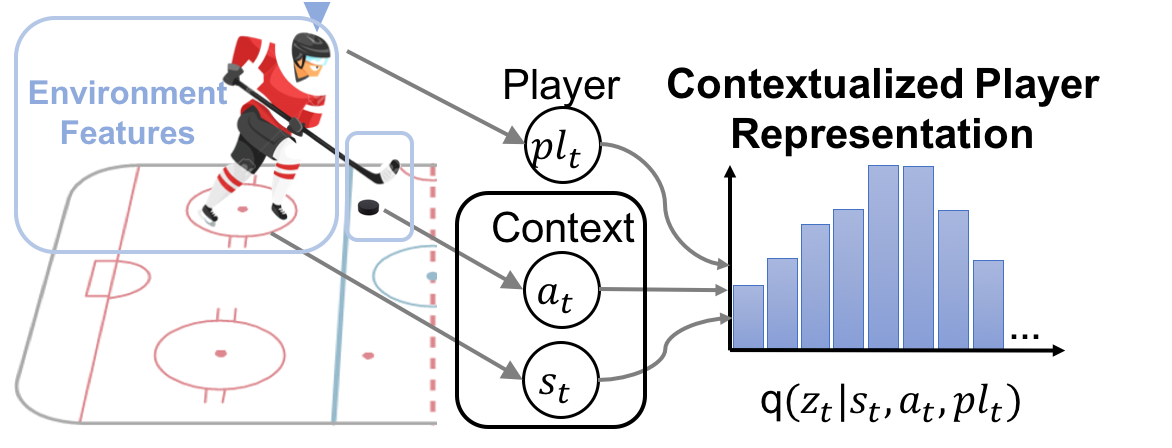
\includegraphics[width=0.45\textwidth] 
    {./figures/player-embedding-example.png}
    \caption{An example of our contextualized player representation, from which we sample the player embeddings.
    } 
    \label{fig:ice-hockey-rink}
\end{figure}

To overcome the limitation, in this work, we build a Variational Hierarchical Encoder with Recurrence (VHER). VHER combines a Bayesian hierarchical model~\cite{kruschke2014doing} and variational inference to embed the player information in latent variables under different game contexts.
The hierarchical model is trained to identify the acting player, where we sample some latent variables from a context-specific prior and compute $N$ (the number of players) Bernoulli distributions to model the presence of each player. The Bernoulli parameters are then normalized for a categorical distribution to predict the current on-the-puck player. 
We then apply variational inference to learn the model parameters. Compared to Monte Carlo Markov Chain (MCMC) and grid approximation, variational inference can generalize well to complex parameter spaces and significantly reduce the learning time under neural network implementation~\cite{BleiKM16}. During the inference, the posteriors for each player are encouraged to shrink toward the mode of the context-specific prior, which substantially reduces the training variance. 
This shrinkage effect in our hierarchical model naturally
% reflects the essence of our contextualized player embedding 
formalizes the idea that “similar players appear in a similar context”. 
We also apply the posterior distribution for each player to predict the current on-the-puck player, which encourages the diversity of the posterior player representations.
% Both the shrinkage effect and embedding diversity are well present in an Evidence Lower Bound (ELBO).
To demonstrate the effectiveness of our player embedding, we apply them to the secondary (embedding) task of identifying the acting player and the external validation task of predicting the expected goal. Experimental results show the improvement of model performance with our player embedding.  


\section{Related Works}
In this section, we introduce the previous works that are most related to our model.

\subsection{Variational Auto-Encoder}
Variational Auto-Encoder (VAE) has achieved promising performance in recovering multimodal distributions and in generating many kinds of complicated data, including hand-writing, faces~\cite{kingma2013auto}, images~\cite{gregor2015draw} and player actions~\cite{mehrasa2019variational}.
VAE applies a set of latent variables $\latentvariables$ to capture the variations of observed variables $\observation$.
During the generative process, the prior of $\latentvariables$ is generally chosen to be a simple Gaussian distribution.
VAE models the likelihood function $\generation(\observation|\latentvariables)$ with a decoder (usually implemented as a Gaussian or Bernoulli Multi-Layer Perceptron (MLP)~\cite{kingma2013auto}, which applies a highly non-linear mapping from $\latentvariables$ to $\observation$.

The non-linearity in complicated likelihood function $\generation(\observation|\latentvariables)$ leads to the intractable inference of the posterior $p(\latentvariables|\observation)$. Instead, VAE approximates the true posterior with a recognition model (decoder) $\inference(\latentvariables|\observation)$, which is usually defined as a Gaussian as $\latentvariables\sim\mathcal{N}[\boldsymbol{\mu}, diag(\boldsymbol{\sigma}^{2})]$ ($\boldsymbol{\mu}$ and $\boldsymbol{\sigma}$ are computed with observed variables $\observation$).
Parameters of both decoder and encoder are optimized by maximizing a lower bound of the marginal likelihood of observation $p(x)$ :
\begin{align}
    % & \log p(x) \geq \mathcal{L}(p(\observation))\\
     \mathcal{L}(p(\observation))&=-KL(\inference(\latentvariables|\observation)||p(\latentvariables))+\mathbb{E}_{\inference(\latentvariables|\observation)}\Big[\log\generation(\observation|\latentvariables)\Big]
\end{align}

~\cite{kingma2013auto} introduced an alternative method for generating samples from $\inference(\latentvariables|\player)$ and described a reparameterizing trick for VAE. By rewriting:
\begin{equation}
    \mathbb{E}\Big[\log(\generation(\observation|\latentvariables))\Big]=\mathbb{E}\Big[\log \generation(\observation|\latentvariables=\boldsymbol{\mu}+\boldsymbol{\sigma}\odot\boldsymbol{\epsilon})\Big]
\end{equation}
where $\boldsymbol{\epsilon}\sim\mathcal{N}(0,1)$, reparameterizing makes the estimations of the expectation with respect to $\inference(\latentvariables|\observation)$ differentiable.

To handle sequential data, \citeauthor{ChungKDGCB15} combined the latent variables with a recurrent model.
The proposed Variational Recurrent Neural Network (VRNN) includes a VAE at every time step $t$. The object function is a timestep-wise variational lower bound:
\begin{align}
    %  \mathcal{L}\Big[\sum_{t=1}^{T}p(x_{t})\Big] = &
     \sum_{t=1}^{T}\Big[-KL(\inference(\latentvariables_{t}|\observation_{\leq t},\latentvariables_{<t})||p(\latentvariables_{t}|\observation_{< t},\latentvariables_{<t}))+
    & \log\generation(\observation_{t}|\latentvariables_{\leq t},\observation_{<t})\Big]
\end{align}

\subsection{Hierarchical Models in Sports Analytics}
% \textcolor{blue}{shall we just name it Bayesian hierarchical model? ,because shrinkage name is not a common name. usually, people call it shrinkage effect in Bayesian hierarchical model.}
Many previous works~\cite{Gelman06,davis2015simulator}
% on shrinkage models 
have built a multi-level hierarchical model and estimated the parameters of the posterior with Bayesian inference.
The Bayesian inference naturally incorporates the shrinkage effect into estimating model parameters. The shrinkage effect pulls the estimates of low-level parameters closer together than they would be if there were not a higher-level distribution, and generally, shrinkage in hierarchical models encourages lower-level parameters to shift toward the modes of the higher-level distribution, which can significantly reduce the variance of estimation. 
Similar hierarchical models have many applications in sports analytics, for example, ~\citeauthor{kruschke2014doing} built a hierarchical model to estimate the batting abilities for individual baseball players.
They sampled the parameters of a likelihood function (modeling players' batting ability by the probabilities of hitting the ball) from a prior conditioning on player position.
Accordingly, for players in the same position, despite the difference in performance, shrinkage toward the position-specific mode leaves the posterior distribution of their difference being nearly zero.
Such a shrinkage effect can facilitate our player embedding model. Given the observation that similar players are likely to appear in similar contexts, our model is trained to dynamically encourage the embedding to shift toward the mode of a context-specific prior.

\subsection{Contextualized Embedding}
As a promising technique of incorporating background knowledge into the object modeling, contextualized embedding have been extensively studied under the topics related to Natural Language Processing, for example, a recent work~\cite{AkbikBV18} proposed a contextual string embedding. The embedding model contextualizes words by their surrounding text. Correspondingly, the same word will have different embeddings depending on its contextual use. A more recent work~\cite{PetersNIGCLZ18} computed the contextualized embedding to model complex characteristics of word use (e.g., syntax and semantics) and extended the application of embeddings across linguistic contexts. They showed the embeddings can be easily added to existing models and significantly improved the state-of-the-art across six challenging NLP problems. To utilize the advantage of contextualized embedding, in this work, we compute the embeddings for NHL players conditioning on different game contexts (including the current observation and play history). Our results also demonstrate the benefit of applying contextualized embeddings in identifying pids and predicting expected goals. 
% \textcolor{blue}{explain why we don't we compare with the word embedding model.}


% \subsection{Agent Representations in RL?} 


% \section{Problem Formulation}
% \textcolor{blue}{Shorten the idea and place it under the introduction.}
% To utilize the player information, we formulate this task into two sub-problems: 1) How to learn a robust player embedding model and 2) How will the embedding influence the mode performance in solving the practical problem.

% For the first problem, we investigate the game environment, actions and games statistic that feature a player's overall playing skill.  
% To include the feature information into our embedding, our model is train to solve a secondary prediction problem: Given the condition a on-the-ball action $\action_{t}$, game context $\state_{t}$ (including locations, game time etc.) and play history $\hiddenstate_{t-1}$, who is likely to be the player   $\player_{t}$ performing the action. In this sense, our model summarizes all the conditional feature information into a embedding vector, and unlike previous works which assigns a deterministic embedding vector to each player, our model learns to generate a comprehensive embedding vector $\latentvariables_{t}$ conditioning on various game or player features. 

% To answer the second question, we look into two commonly studied problems including 1) game outcome prediction and 2) player performance evaluation. 
% In the recent years, many works have applied machine learning models to solve those problems, but a common drawback of the proposed models is they considered very limited player information.
% To overcome the limitation and validate our conditional embedding,
% % demonstrate the benefit of adding more player information
% , we input the learned player embedding vectors into their model and check whether and how the embedding will improve the model performances. 


\section{Modeling Play Dynamics}
\subsection{Dataset}
We utilize a dataset constructed by SPORTLOGiQ with computer vision techniques. 
% including player tracking and activity recognition. 
% It consists of play-by-play information of game events and player actions for the entire 2015-2016 NHL season. 
The data provide information about \textbf{game events} and \textbf{player actions} for the entire 2018-2019 NHL (largest professional ice hockey league) season,
which contains over 4 million events, covering 31 teams, 1,196 games and 1,003 players. 
% Table \ref{table:example-of-dataset} shows an excerpt. 
% A breakdown of this dataset is shown in table \ref{table:size-of-dataset}. 
% \begin{table}[htbp]
% \caption{Dataset Statistics.}
% \label{table:size-of-dataset}
% \begin{center}
% \begin{tabular}{|l|c|}
% \hline
% \bf{Number of Teams} & xx \\ \hline
% \bf{Number of Players} & x,xxx \\ \hline
% \bf{Number of Games} & x,xxx \\ \hline
% \bf{Number of Events} & x,xxx,xxx \\ \hline
% \end{tabular}
% \end{center}
% \end{table}
The data track events around the puck, and record the identity and actions of the player in possession, with space and time stamps, as well as features of the game context. 
% We used 13 of the recorded action types listed in the supplementary material.
The table utilizes adjusted spatial coordinates where negative numbers refer to the defensive zone of the acting player, positive numbers to his offensive zone. Adjusted X-coordinates run from -100 to +100, Y-coordinates from 42.5 to -42.5, where the origin is at the ice center as in Figure~\ref{fig:ice-hockey-rink}. We augment the data with derived features
and list the complete feature set in Table \ref{table:feature-of-dataset}.

% \begin{table}[htb]
% % \caption{Complete Feature List}
% % \label{table:feature-of-dataset}
% \begin{center}
% \resizebox{\columnwidth}{!}{
% \begin{tabular}{|c|c|c|}
% \hline
% \bf{Name} & \bf{Type} & \bf{Range} \\ \hline
% X Coordinate of Puck & Continuous & [-100, 100]\\
% Y Coordinate of Puck & Continuous & [-42.5, 42.5]\\
% Velocity of Puck & Continuous & (-inf, +inf)\\
% Game Time Remain & Continuous & [0, 3600]\\
% Score Differential & Discrete & (-inf, +inf)\\
% Manpower Situation & Discrete & \{EV, SH, PP\}\\
% Event Duration & Continuous & [0, +inf) \\
% Action Outcome & Discrete & \{successful, failure\}\\
% Angle between puck and goal & Continuous & [$-3.14$, $3.14$]\\
% Home or Away Team & Discrete & \{Home, Away\} \\ \hline
% \end{tabular}
% }
% \end{center}
% \caption{Complete Feature List}
% \label{table:feature-of-dataset}
% \end{table} 

\begin{table}[]
\begin{tabular}{c|c|c}
\hline
Type & Name & Range \\ \hline
\multirow{5}{*}{\begin{tabular}[c]{@{}c@{}}Spatial \\ Features\end{tabular}} & X Coordinate of Puck & {[}-100, 100{]} \\
 & Y Coordinate of Puck & {[}-42.5, 42.5{]} \\
 & Velocity of Puck & $(-\infty,+\infty)$ \\
 & Angle between & \multirow{2}{*}{\begin{tabular}[c]{@{}c@{}}[$-3.14$, $3.14$] \end{tabular}}\\ 
 & the puck and the goal & \\
 \hline
\multirow{2}{*}{\begin{tabular}[c]{@{}c@{}}Temporal \\ Features\end{tabular}} & Game Time Remain & ($-\infty$, 3,600{]} \\
 & Event Duration & (0, $+\infty$) \\ \hline
\multirow{4}{*}{\begin{tabular}[c]{@{}c@{}} In-Game \\ Features\end{tabular}} & Score Differential & $(-\infty,+\infty)$ \\
 & Manpower Situation & \{EV, SH, PP\} \\
 & Home or Away Team & \{Home, Away\} \\
% \multirow{2}{*}{\begin{tabular}[c]{@{}c@{}}Action\\ Type\end{tabular}} & Action Name & One-hot-vector \\
 & Action Outcome & \{successful, failure\} \\ \hline
Pre-game & \multirow{2}{*}{\begin{tabular}[c]{@{}c@{}}Box Score\end{tabular}} &\multirow{2}{*}{\begin{tabular}[c]{@{}c@{}}$(-\infty,+\infty)$\end{tabular}}\\  Statistics &  & \\
\hline
\end{tabular}
\caption{Complete Feature List. 
% * indicates the external data\footnote{http://www.nhl.com/stats/}. 
We have experimented with the option of incorporating players' box scores into our embedding. The box score includes players' pre-games cumulative statistics: The total number of goals, assists, points, penalty minutes, and played games from the beginning of the 2017-18 NHL season to the beginning of the current game. }
\label{table:feature-of-dataset}
\end{table}

\subsection{Contextual Variables for NHL Players}
In the SPORTLOGiQ dataset, the play dynamics is captured by contextual variables as follows:
\begin{itemize}
\item The \textbf{action} $\action_t$ records the movements of players who control the puck. Our model applies a discrete action vector with the one-hot representation. 
\item The \textbf{environment variables} $\features_{t}$ describes the game environment where the action is performed. We represent it as a feature vector specifying a value of the features listed in Table~\ref{table:feature-of-dataset} at a discrete-time step $t$. 
% We use the complete sequence $\state_{t} \equiv (\features_t,\action_{t-1},\features_{t-1},\ldots,\features_0)$ to represent the game \textbf{state} \cite{Mnih2015}.
\end{itemize}

In each game, we consider event data of the form
$\features_0,\player_0,\action_0,\features_1,\player_1,\action_1,\ldots,\features_{t},\player_{t},\action_{t},\ldots$:
% $\features_0,\player_0,\action_0,\reward_1,\features_1,\player_1,\action_1,\ldots,\features_{t-1}, \player_{t-1}, \action_{t-1}, \reward_{t},\features_{t},\action_{t}$
at time $t$, after observing environment $\features_{t}$, player $\player_{t}$ takes a turn (possesses the puck) and chooses an action $\action_{t}$.
% , resulting in a reward $\reward_{t}$. 
% At the next time step, given the observed features $\features_{t}$, another action $\action_{t}$ is chosen, etc. In a sports application (like hockey), $\player_t$ taking a turn means that $\player_t$ gains possession (of the puck).
% \textcolor{blue}{Guess we'd better include the time t, if we start by introducing the temporal event dataset. I can do it if you agree}
The observations for a given player $\pindex$ 
form a set of triples $(\player_{t} = \pindex, \state_{t}, \action_{t})$, where to alleviate the partial observability in the dataset, the game state $\state_{t}$ includes the game history $\state_{t} \equiv (\features_t,\action_{t-1},\features_{t-1},\ldots,\features_0)$ \cite{Liu2018,littlestone}.
Each triple summarizes the observed player actions and the game environment, with a joint distribution $\generation(\player_{t}, \state_{t}, \action_{t})$. This distribution can be factored into two components:
% , only one of which is related to the player:

\begin{equation}
    \label{eq:player-factor} 
    \generation(\player_{t}, \state_{t}, \action_{t}) = \generation(\player_{t}|\state_{t},\action_{t}) \generation(\state_{t},\action_{t}).
\end{equation}

\noindent where the player-independent component $\generation(\state_{t},\action_{t})$ represents the game context (observed action and state at $t$) and $\generation(\player_{t}|\state_{t},\action_{t})$ models the dependency between the observed game context and the acting player $\player_{t}$.
The second component describes a player tendency to act under different game states, which makes it an appropriate target for learning contextualized embedding for each player. 

% \begin{itemize}
    % \item There are two agents, $\home$ and $\away$, representing their respective teams. \textcolor{blue}{shall we mention two agents here?}
    % \item The \textbf{action} $\action_t$ records the movements of players who control the ball. Our model applies a discrete action vector with the one-hot representation.
    %We write $\action_{t,\home}$ to indicate that an action is taken by the home team, and similarly for the away team. 
    % During training, actions are represented as a one-hot vector $\action_t$, whose dimension equals to the size of action spaces.
    % \item An \textbf{observation} is a feature vector $\features_{t}$ specifying a value of the features listed in Table~\ref{table:feature-of-dataset} at a discrete time step $t$. We use the complete sequence $\state_{t} \equiv (\features_t,\action_{t-1},\features_{t-1},\ldots,\features_0)$ to represent the \textbf{state} \cite{Mnih2015}.
    % , which satisfies the Markov property.
    % \item The \textbf{reward} $\reward_{t}$ is a vector of goal values $\goal_t$ that specifies which team ($\home,\away$) scores. 
    % We introduce an extra $\none$ indicator for the eventuality that neither team scores until the end of a game.
    % For readability, we use $\home,\away,\none$ to denote the team in a 1-of-3 vector of goal values  $\reward_{t}=[\goal_{t,\home}, \goal_{t,\away}, \goal_{t,\none}]$ and $\goal_{t,\home}=1 $ indicates the home team scores at time $t$~\textcolor{blue}{Maybe we should include reward into our condition}. 
% \end{itemize}


\section{Contextualized Player Representation}
We introduce our novel Variational Hierarchical Encoder with Recurrence (VHER) which combines a generative Bayesian hierarchical model with variational inference for obtaining a contextualized player Representation. 

\subsection{Bayesian Hierarchical Model}

To model the player-related component $ \generation(\player_{t}|\state_{t},\action_{t})$, we build a {\em Bayesian hierarchical model}, shown in  Figure~\ref{fig:hierarchical-model}, where parameters are assigned distributions like random variables~\cite{McCallum1998,kruschke2014doing}. Our hierarchical model splits $ \generation(\player_{t}|\state_{t},\action_{t})$ into different components:
$$% & \generation(\player_{t}|\state_{t},\action_{t}) \\ 
\sum_{\BernoulliParameters_{\pindex,t}}\big[\generation(\player_{t}|\BernoulliParameters_{\pindex,t})\generation(\BernoulliParameters_{\pindex,t}|\latentvariables_{t},\state_{t},\action_{t})\big]\generation(\latentvariables_{t}|\GaussianParameters_{t,0})\generation(\GaussianParameters_{t,0}|\state_{t},\action_{t})\nonumber
$$


\begin{figure}[t]
    \centering
    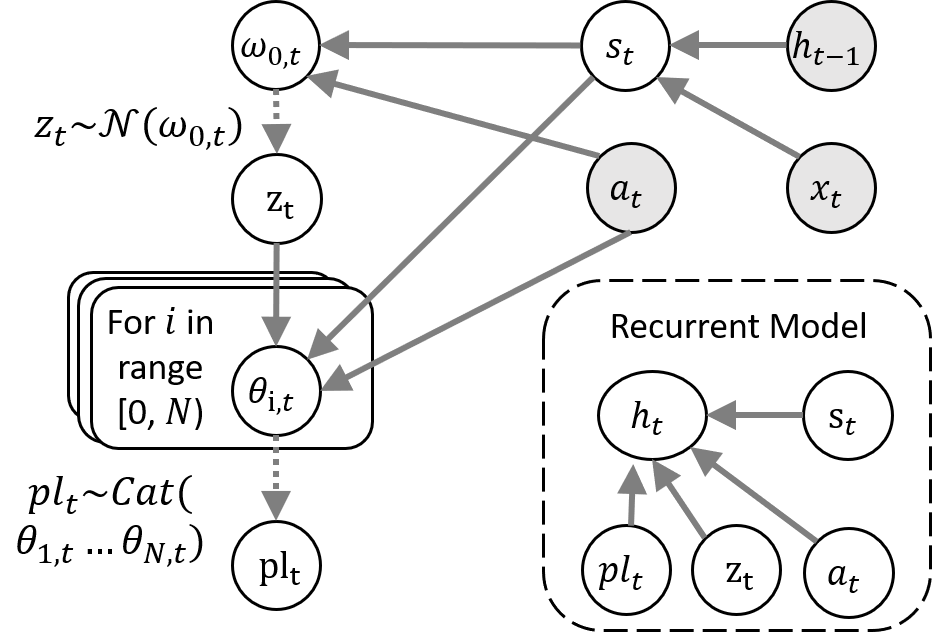
\includegraphics[width=0.8\columnwidth] 
    {./figures/hierarchical-model-graph.png}
    \caption{Graphical illustration of our hierarchical model. Thick (bold) line indicates logical function while thin line denotes stochastic dependence. The shaded nodes are given during generation. Our model applies hidden states $\hiddenstate_{t-1}$ of a LSTM cell to capture the temporal dependence of a series of previously observed environment features and actions, so we represent the state as $\state_t \equiv (\features_{t},\hiddenstate_{t-1})$ and update the hidden states by $\hiddenstate_{t}=f(\features_{t},\action_{t},\latentvariables_{t},\hiddenstate_{t-1})$. $N$ is the number of embedded players.
    } 
    \label{fig:hierarchical-model}
\end{figure} 

Figure~\ref{fig:hierarchical-model} presents a graphical illustration of our hierarchical model.
Conditioning on game context (state-action pair  $\state_{t},\action_{t}$), the prior on the player embeddings (the latent random variables) is represented by a Gaussian distribution:
\begin{align}
    &\boldsymbol{\GaussianParameters}_{0,t} :=\psi^{prior}[\psi^{\context}(\state_{t},\action_{t})]\\
    &\latentvariables_{t}\sim p(\latentvariables_{t}|\state_{t},\action_{t}) \equiv \mathcal{N}(\boldsymbol{\GaussianParameters}_{0,t})\label{eqn:prior}
\end{align}
where $\GaussianParameters_{0,t}\equiv[\boldsymbol{\mu}_{t,0},diag(\boldsymbol{\sigma}_{t,0})]$ denotes the parameters of the context-specific Gaussian prior. 
% \textcolor{red}{Should that be boldface $\mathbf{\mu}$ and $\mathbf{\sigma}$? Also, is the Gaussian isotropic (diagonal covariance) as you discussed in the Related work section?}
A neural network is trained to compute the parameter estimates by implementing 
%To derive those parameters, we implement 
a context function $\psi^{\context}$ that extracts context features and a prior function $\psi^{prior}$ to compute $\boldsymbol{\GaussianParameters}_{0,t}$ from the extracted features. 
% The conditional prior of player embeddings is $\latentvariables_{t} | \state_{t},\action_{t} \equiv \expect_{\latentvariables_{i,t}\sim p(\latentvariables_{i,t}| \state_{t},\action_{t})}(\latentvariables_{i,t})$.

Given the sample latent variables $\latentvariables_{t}$ and game context $(\state_{t}.\action_{t})$, our model generates the label of the on-the-puck (possessing the puck) player as follows:  
\begin{align}
%  \latentvariables_{t} & = (\latentvariables_{1,t},\ldots,\latentvariables_{N,t})\\
        %\text{where } 
    \BernoulliParameters_{\pindex,t}&:=\sigmoid\{\psi^{dec}[\psi^{z}(\latentvariables_{t}), \psi^{\context}(\state_{t},\action_{t})]\} \\
    \player_{t}| \latentvariables_{t}, \state_{t},\action_{t} &\sim Categorical[\softmax(\BernoulliParameters_{1,t},\dots,\BernoulliParameters_{N,t})]
    %\text{ and} \\
   % \softmax(\boldsymbol{x}_{k})&=\exp{(\boldsymbol{x}_{k})}/\sum_{j=1}^{k}\exp{(\boldsymbol{x}_{j})}
\end{align}

\noindent where $\BernoulliParameters_{\pindex,t}$ denotes the parameters of Bernoulli distributions to model the presence of player $\player_{\pindex,t}$. These parameters are computed as follows: (1) A neural network implements the player embedding function $\psi^{z}$ to extract features from the player representations $\latentvariables_{t}$ (2) another neural network implements the context embedding function $ \psi^{\context}(\state_{t},\action_{t})$ to extract features from the game context. (3) The extracted features are input to a decoder function $\psi^{dec}$, whose outputs are mapped to [0,1] by a sigmoid function $\sigmoid$ to compute Bernoulli parameters for each player $i$. (4) The softmax function $\softmax$ normalizes the Bernoulli parameters %($\sum\softmax(\BernoulliParameters_{1,t},\dots,\BernoulliParameters_{N,t})$={\bf 1}) for the following 
to obtain a categorical distribution over players acting at time $t$.

% By estimating the model parameters, we learn a contextualized player representation $\latentvariables_{i,t}|\player_{t}, \state_{t},\action_{t}$ = $\generation(\latentvariables_{i,t}|\GaussianParameters_{t,0},\state_{t},\action_{t})\generation(\GaussianParameters_{t,0}|\state_{t},\action_{t})$.


\subsection{Variational Inference}

% \textcolor{blue}{Maybe instead of naming it VAE, we should call it variational inference conditioning game context for the hierarchical model.} \textcolor{red}{Why not "hierarchical VAE"?}

We apply variational inference to derive an objective function for estimating the parameters of our hierarchical model. The inference is similar to that of Variational Auto Encoder (VAE)~\cite{kingma2013auto}, because both models utilize a prior and approximate posterior on the latent variables to define an approximate log-likelihood function for the observed data. 
% and fit them to a generator to predict the observation ($\player_{t}$ under our player embedding task) 2) define an approximate posterior on the latent variables and compute the parameters during inference. 
The main difference is that our hierarchical model conditions on the game context. In particular, the latent variable prior is learned to be a function of the game context, rather than a context-independent standard distribution.

Figure~\ref{fig:model-struct} illustrates the inference process of our model. After observing the $\player_{t}$, the approximate posterior on a player embedding follows the equation:

\begin{align}
& \boldsymbol{\GaussianParameters}_{\pindex,t}:=\psi^{enc}[\psi^{\player}(\player_{t}),\psi^{\context}(\state_{t},\action_{t})]\\
& \latentvariables_{t} \sim \inference(\latentvariables_{t} |\player_{t} = \pindex,\state_{t},\action_{t}) \equiv \mathcal{N}(\boldsymbol{\GaussianParameters}_{\pindex,t})\label{eqn:approximate-posterior}
\end{align}

% Figure~\ref{fig:model-struct} illustrates the inference process of our model. After observing the $\player_{t}$, the approximate posterior on player embedding follows the equations:

% \begin{align*}
% & \latentvariables_{\player_{\pindex},t}| \player_{\pindex,t}, \state_{t},\action_{t} \equiv  \latentvariables_{\pindex,t}| \player_{\pindex,t}, \state_{t},\action_{t} \sim  \mathcal{N}(\boldsymbol{\GaussianParameters}_{\player_{\pindex},t})\\ 
% & \text{ where }  \boldsymbol{\GaussianParameters}_{\player_{\pindex},t}=\psi^{enc}[\psi^{\player}(\player_{\pindex,t}),\psi^{\context}(\state_{t},\action_{t})]
% \end{align*}

\noindent where we apply neural networks to implement (1) a observation function $\psi^{\player}$ that extracts features from  $\player_{t}$ (represented as an one-hot vector of $N$ dimensions)
%and $\player_{\pindex,t}$ denotes the value in $\pindex^{th}$ dimension) 
(2) a context function $\psi^{\context}$ that extract features from game context ($\state_{t},\action_{t}$), and (3) an encoding function $\psi^{enc}$ generates the parameters $\boldsymbol{\GaussianParameters}_{\pindex,t}\equiv[\boldsymbol{\mu}_{\pindex,t},diag(\boldsymbol{\sigma}_{\pindex,t})]$ of an approximate Gaussian posterior, with which we sample embeddings of individual players.
% We use 
% $\latentvariables_{\player_{\pindex},t}| \player_{\pindex,t}, \state_{t},\action_{t} \equiv  \latentvariables_{\pindex,t}| \player_{\pindex,t}, \state_{t},\action_{t}$
% % $\latentvariables_{\player,t} | \player_{t}, \state_{t},\action_{t} \equiv \expect_{\latentvariables_{\player_{\pindex},t}\sim q(\latentvariables_{\player_{\pindex},t}|\player_{\pindex,t}, \state_{t},\action_{t})}(\latentvariables_{\pindex,t})$ %. % \equiv \latentvariables| \player, \state,\action$ %
% %
% to emphasize that the code for the approximate posterior is associated with a specific observed player $\player_{t}$. 
The posterior $\inference(\latentvariables_{t} |\player_{t}=\pindex,\state_{t},\action_{t})$ is used as a 
representation for player $\pindex$, with which we can construct a context-dependent embedding vector. This real-valued vector can replace the one-hot player representation and facilitate downstream application such as expected goal or game outcome prediction.

\begin{figure}[htbp]
    \centering
    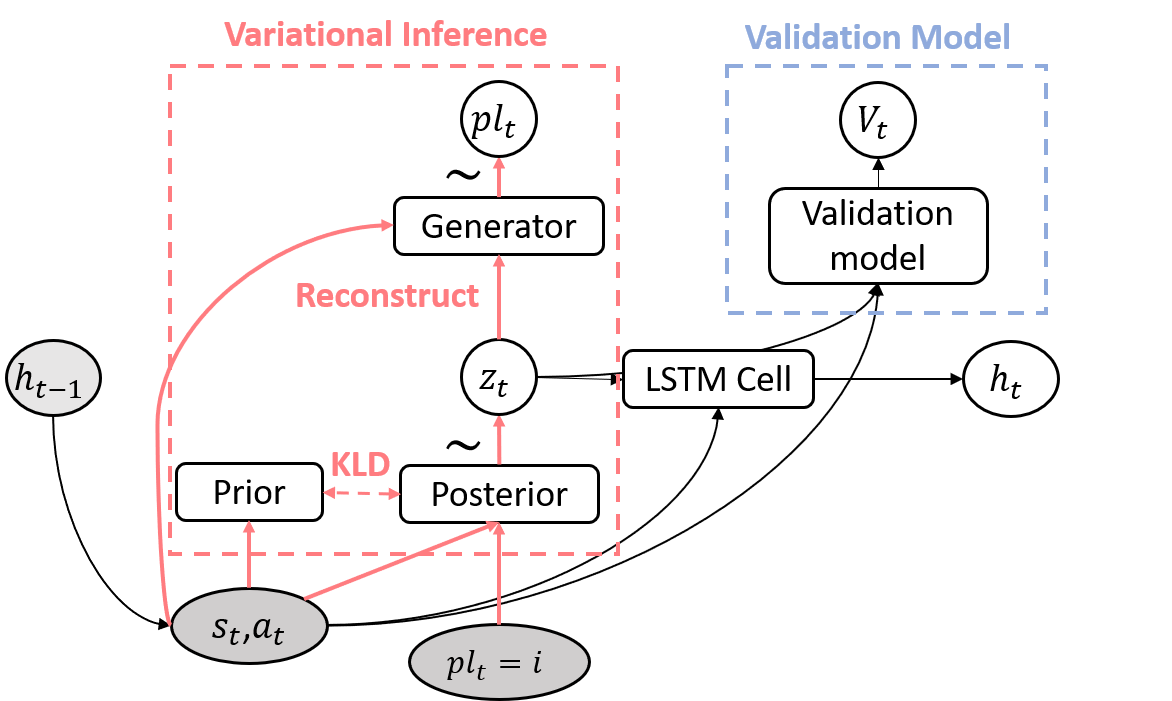
\includegraphics[width=1\columnwidth] 
    {./figures/cvrnn_structure.png}
    \caption{Learning the player representations and applying them to the validation model. The prior and the posterior respectively represent the Gaussian Prior and the approximate posterior of latent variables, with which the generator reconstructs $\player_{t}$. Red arrows indicate the process of variational inference, and the shaded nodes are given during training.
    } 
    \label{fig:model-struct}
\end{figure} 

% \paragraph{Learning} 
Based on the time-wise variational lower bound~\cite{ChungKDGCB15}, the loss function for player embedding model is
% the ELBO objective for generating a player ID at time $t$:

\begin{align} \label{eq:loss}
        &\sum_{t=1}^{T}\Big\{ KL\Big[\inference(\latentvariables_{t} |\player_{t} = \pindex,\state_{t},\action_{t})||\prior(\latentvariables_{t}|\state_{t},\action_{t})\Big]-\\
        % &\expect_{\inference(\latentvariables_{\player,t} |\player_{t},\state_{t},\action_{t})}
        &\expect_{\latentvariables_{t}|\player_{t},\state_{t},\action_{t}}
        \Big[\log\generation(\player_{t}|\latentvariables_{t},\state_{t},\action_{t}) -\lambda^{V}
        \mathcal{L}^{V}( \latentvariables_{t},\state_{t},\action_{t})\Big]
        \Big\} \nonumber
\end{align}

% \begin{align*}
%         % \log&\Big[p(\player_{\leq t}|\context_{\leq t})\Big] \\
%         % \geq
%         & \expect_{\inference(\latentvariables_{\player} |\state,\action,\player)} \Big\{KL\Big[\inference(\latentvariables_{\player} |\player,\state,\action)||\prior(\latentvariables_{0}|\state,\action)\Big]-\\
%         &\log\Big[\generation(\player|\latentvariables_{\player},\state,\action)\Big] -\lambda^{V} \mathcal{L}^{V}( \latentvariables_{\player},\state,\action)
%         \Big\}
% \end{align*}
\noindent where we add a validation loss $\mathcal{L}^{V}$ with a parameter $\lambda^{V}$ to control its scale. This loss combines the gradient of the validation model into the embedding inference and dynamically incorporates player embeddings into different applications. 



% \textcolor{red}{Also need to clarify what we take the player representation to be. E.g. the approximate posterior distribution $\inference$ as represented by its parameters, or a sample of size $k$ from the approximate posterior distribution?}

\subsection{Interpretation and Motivation}

We provide two interpretations of the hierarchical VAE model that in our view show why this is a good model for representing the available statistical information about a player. 

\paragraph{Predictive Model}
% \textcolor{blue}{maybe named it as a secondary task and we will a have a reference.}
Viewed as a predictive model, our VHER solves the {\em re-identification task}~\cite{LaviRID2018}: identifying which player is currently acting given a history of events. For example, a computer vision system may try to identify a player's jersey number from video footage. As Equation~\eqref{eq:player-factor} shows, this task captures the correlations between the identity of a player, and what they do in which match contexts. The prior distribution $\prior(\latentvariables_{t}|\state_{t},\action_{t})$ can be seen as representing the probability  that a randomly chosen player acts in a given game context. 
% cold-start probability that a new player acts in a given game context. \textcolor{red}{Or also: the probability that a randomly chosen player acts in a given game context. Which do you prefer?}
Our experiment also studies the predictive of performance of VHER.

\paragraph{Shrinkage Effect}
A hierarchical model is commonly used in statistics to capture similarities among a group of individuals ~\cite{McCallum1998,kruschke2014doing}.  The intuition motivating hierarchical models is that {\em statistically similar agents are assigned similar representations}. Previous hierarchical models have been constructed for parametric models, which estimate a separate parameter vector for each player~\cite{Murphybook12}. Parametric hierarchical models achieve a {\em shrinkage effect} where the differences between different parameter vectors for each individual are shrunk towards a common value. Shrinkage estimators have strong statistical properties because they allow information to be transferred between the observations of different individuals. 
In a Bayesian hierarchical model, shrinkage is achieved by estimating the individual agent parameters using the posterior distribution over parameters drawn from a common prior for the group. 

As Equation~\eqref{eq:loss} shows, the VAE loss function induces a shrinkage effect by regularizing the approximate posterior for each individual player towards a common prior $\prior(\latentvariables_{t}|\state_{t},\action_{t})$. The Conditional VAE, in fact, achieves a {\em joint} shrinkage effect where {\em statistically similar agents are assigned similar representations in similar contexts.} This is because we can interpret the prior distribution $\prior(\latentvariables_{t}|\state_{t},\action_{t})$ as a joint representation of the player's action and game context: After training, state-action pairs that tend to feature the same players will be associated with similar prior distributions. In sum, we have described a non-parametric hierarchical CVAE model that generates dynamic context-aware player representations with a joint shrinkage effect for players, actions, and game states. 

\section{Empirical Evaluation}

\subsection{Experiment Setting}
\paragraph{Training settings:}
We divide the dataset containing 1,196 games into a training set (80\%), a validation set (10\%) and a testing set (10\%). Our model is implemented in Tensorflow. The total number of player ($N$) is 1,003. The dimension of the player embedding as well as the dimension of parameters in Gaussian Prior and Posterior are set to 256.

\paragraph{Baseline models:}
% To demonstrate the advantage of embedding generated by our Bayesian hierarchical model, 
Our first baseline model is a Deterministic Encoder (DE) model~\cite{ganguly2018problem}. It is trained as a regressor to identify the acting player and implements a deterministic projection from the game context to player embedding (a middle layer of the neural network) without modeling the prediction uncertainty (or variance). The second baseline model is a Conditional Variational Auto-Encoder (CVAE)~\cite{wal}. Compared to our VHER, CVAE conditions the player representation on current game observation, which does not incorporate the play history into embedding computation. 
% \textcolor{red}{So is CVAE = VHER - Recurrence? Perhaps just call it VHE then.} 
To study the influence of player embedding, we also include an LSTM as our third baseline model. LSTM directly finishes the experimented tasks without including any player information.


% \textcolor{red}{how about hyperparameters for our model?}


\subsection{Identify the Acting Player}
Similar to~\cite{ganguly2018problem}, to learn the player representation, our VHER is trained for a secondary task of predicting the acting (on-the-ball) player given the game context ($\state_{t},\action_{t}$), so this experiment studies the performance of VHER as a predictive model and compares it with the other three baseline models.
To assess alternative ways of including player information, we also experiment with the options of including players' pre-game cumulative box score (see table~\ref{table:feature-of-dataset}) into game context.

% \begin{table}[t]
% \centering
%     \begin{tabular}{c|cc}
%     \hline
%      \multirow{2}{*}{\begin{tabular}[c]{@{}c@{}}Prediction\\ Method\end{tabular}} & \multicolumn{2}{c}{Performance (No  Box-Scores)} \\ \cline{2-3}
%      & ACC & LL \\ \hline \hline
%     DE & 11.20 \% $\pm$ 0.00 & -19.757 $\pm$ \\
%     CVAE &  9.40 \% $\pm$  & -4.927 $\pm$\\
%     VHE & 10.52 \%  $\pm$ & -4.917 $\pm$ \\
%     LSTM & 12.48 \% $\pm$ & -3.114 $\pm$ \\
%     VHER & 48.12 \% $\pm$ & -2.075 $\pm$ \\ \hline
%     \end{tabular}
%     \caption{Results for player identification. Acc=Accuracy and LL=Log-Likelihood.}
%     \label{table:exp-pid}
% \end{table}

% \begin{table}[t]
% \centering
%     \begin{tabular}{c|cc}
%     \hline
%      \multirow{2}{*}{\begin{tabular}[c]{@{}c@{}}Prediction\\ Method\end{tabular}} & \multicolumn{2}{c}{Performance (With Box-Scores)} \\ \cline{2-3}
%      & ACC & LL \\ \hline \hline
%     DE & 22.98 \% & -17.059 \\
%     CVAE &   29.30 \% &  -4.730 \\
%     VHE &  36.43 \% &  -4.658  \\
%     LSTM &  61.76 \% &  -1.695 \\
%     VHER &  83.41 \% &  1.674 \\ \hline
%     \end{tabular}
%     \caption{Results for player identification. Acc=Accuracy and LL=Log-Likelihood.}
%     \label{table:exp-pid}
% \end{table}

\begin{table}[t]
\centering
    \begin{tabular}{c|cc|cc}
    \hline
     & \multicolumn{2}{c|}{No Box Score} & \multicolumn{2}{c}{With Box Score} \\ \hline
    Method & ACC & LL & ACC & LL \\ \hline
    DE & 10.91 \% & -19.482 & 14.85 \% & -18.590 \\
    CVAE & 7.42 \% & -4.294 & 17.21 \% & -4.850 \\
    % VHE &  &  &  &  \\
    LSTM & 12.41\% & -3.131 & 64.47\% & -1.718 \\
    VHER & 48.00 \% & -2.228 & 82.13\% & -1.402 \\ \hline
    \end{tabular}
    \caption{Results for player identification. Acc=Accuracy and LL=Log-Likelihood.}
    \label{table:exp-pid}
\end{table}

Table~\ref{table:exp-pid} shows the experimental results. Predictions from DE have a significantly lower log-likelihood than the other three methods. 
It is because trained as a standard regression model, the DE objective minimizes the distance between a single prediction and the ground truth. This method, however, will fail if the output space is multi-modal.
% , and thus creates a large training variance. 
% and thus achieves very limited performance. 
% \textcolor{red}{It's okay but it would be nice if it were clearer. Is this the uni-modal vs. multi-modal prediction issue? Also should be clear on which variance we are talking about $p(z)$, $p(x|z)$, $q(z|x)$...}
To handle it, variational models compute multiple isotropic Gaussian priors (Equation~\ref{eqn:prior}) on the latent variables which creating a disentangled representations for each player, and thus facilitates the modeling of multiple modes.
It explains why CVAE manages to improve the log-likelihood. The performance of CVAE is still limited by the lack of game information. To study the influence of incorporating play history, we directly apply a LSTM to identify the acting player and  achieve a better performance. 
Compared to the above baseline models, our VHER utilizes the advantage of both CVAE and LSTM: shrinkage toward a context-specific prior and incorporating play history. 
% \textcolor{red}{Does CVAE or VHE include a common prior and shrinkage effect as well? See question above.}
Therefore, VHER, achieves a significant increase of prediction accuracy and log-likelihood over other baseline methods. We also find including the box score will further improve the performance. This is because the box-scores provide a strong prior for identifying the acting player. 
% The model can easily determine the ability of a player without looking at game data. \textcolor{red}{Do you mean "identity" or "ability". Also, this does not seem to be easy for the CVAE. Kind of strange. Maybe omit this sentence}

\subsection{Predict the Expected Goal}

% \textcolor{red}{Need to explain any preprocessing or special training done for unbalanced data. With a reference to previous work if it exists.}
In this section, we validate the player embeddings in a practical task of predicting the Expected Goal (EG).
Expected Goal (EG) weights each shot by the chance of it leading to a goal. To see if the embeddings will improve the prediction accuracy of EG, we generate the player embedding $\latentvariables_{t}$ for the on-the-ball player $\player_{t}$.
As Figure~\ref{fig:model-struct} shows, at time $t$, we input $\state_{t},shot_{t},\latentvariables_{t}$ to a validation model, which, similar to a classifier, is trained to generate 1 if a goal is scored after the player $\player_{t}$ makes the shot and 0 otherwise. 

We refer to a neural net for the validation task as the validation model. Our validation model is an LSTM that is given the play history, combined with three comparison methods of including current-player information: 1) our dense VHER embeddings, 2) directly inputting one-hot player ids (Pids), 3) no player information. 
% (e.g. VHER) and with Dense layers otherwise (e.g. Encoder and CVAE). 
% To investigate the advantage of continuous-value embedding vectors for players, we also evaluate comparison methods including apply no player information ($\emptyset$) and directly inputting player ids (Pids) into the validation model.
To train the validation model, we utilized the game context for action shot recorded in our NHL dataset and supervise the training by whether the shot will lead to a goal in real games. However, considering that most of the shots will not score any goals, the training data is highly imbalanced.
% , which will encourage the model to label all the shots as 0, in order to %improve the overall prediction accuracy. 
We handle the imbalance with a resampling method~\cite{good2006resampling} so that equal numbers of success and failed shots are included in the training dataset. 


\begin{table}[htbp]
    % \end{minipage}\par\bigskip
    % \begin{minipage}[t]{1\columnwidth}
    \centering
        % \begin{tabular}{ccccc}
        % \hline
        % Model & P & R & F1 & LL  \\ \hline
        % LSTM & 0.144 & 0.808& 0.245 & -0.641 \\
        % Pid+LSTM & 0.103 & 0.691 & 0.179 & -0.573 \\
        % Encoder+LSTM & 0.206 & 0.788 & 0.326 & -2.756 \\
        % CVAE+LSTM & 0.252 & 0.939 & 0.397 & -2.589 \\
        % VHER+LSTM & 0.624 & 0.846 & 0.718 & -0.281  \\
        % % VHER+LSTM+Box & 0.593 & 0.849 & 0.698 & -0.380 \\ 
        % \hline
        % \end{tabular}
        \begin{tabular}{c|cccc}
        \hline
        Model & \multicolumn{4}{c}{Metric} \\ \hline
        Player Info  & P & R & F1 & LL \\ \hline
         N/A  & 0.144 & 0.808& 0.245 & -0.641  \\
        Pids  & 0.103 & 0.691 & 0.179 & -0.573 \\
        DE  & 0.206 & 0.903 & 0.335 & -2.756 \\
        CVAE  & 0.252 & 0.939 & 0.397 & -2.589 \\
        % VHE & LSTM &  &  &  & \\
        VHER  & 0.624 & 0.846 & 0.718 & -0.281  \\ \hline
        \end{tabular}
        \caption{Results for predicting the Expected Goal. The evaluation metrics include Precision (P), Recall (R), F1-score and Log-Likelihood (LL). }
        \label{table:exp-eg}
    % \end{minipage}
    % }
\end{table}

Table~\ref{table:exp-eg} shows the results on the testing set. Without including any player information, predictions from a LSTM model have large recall but very limited precision. Thus the model prefers labeling many shots as goals, but most of the predictions are incorrect. This problem has not been alleviated after adding the pids to the input space, which shows it is hard to utilize the player information with only a sparse one-hot label. Providing more useful player information, DE deterministically maps the player information into a dense player embedding vector and CVAE further improves the embedding with the latent variables. A common problem for the above embedding methods is the absence of play history during training. To overcome this limitation, our VHER applies a recurrent model to fit the play history and substantially improves the precision of predictions. 
% \textcolor{red}{this sounds as if adding recurrence to DE during embedding would fix most of the problems. Something for future work?}
% We also experiment applying box score \textcolor{blue}{more results to be include}

%would be interesting to know the accuracy on unprocessed test set data

% \begin{table}[htbp]
% \begin{tabular}{ccccc}
% \hline
% Model & TP & FP & TN & FN \\ \hline
% LSTM & 572 & 3,389 & 13,109 & 136 \\
% LSTM+Pid & 489 & 4,269 & 12,229 & 219 \\
% Encoder+Dense & 360 & 2,278 & 14,220 & 348 \\
% CVAE+Dense & 670 & 2,073 & 14,425 & 38 \\
% CVRNN+LSTM & 618 & 609 & 15,889 & 90 \\
% CVRNN+LSTM+Box & 608 & 405 & 16,093 & 100 \\ \hline
% \end{tabular}
% \caption{The detailed results of Expected Goal experiment.}
% \end{table}


% \subsection{Predict the estimated probability of scoring the next goal} 
% \textcolor{blue}{ Previous evaluations work only on action shot, and current evaluations are for all actions.}
% We compute Q values to estimate the probability of scoring the next goal within different states of a NHL game. Following ~\cite{Liu2018}, we divide a NHL game into {\bf goal-scoring episodes}, so that each episode 1) starts at the beginning of the game, or immediately after a goal, and 2) terminates with a goal or at the end of the game. 
% A goal-scoring episode contains sufficient information about both offensive and defensive movements of players in home and away team.
% In a goal-scoring episode, the Q values estimated the probability that the home resp. away team {\em scores the goal at the end of the current goal-scoring episode} ($\egoal_{\home}=1$ resp. $\egoal_{\away}=1$), or neither team scores ($\egoal_{\none}=1$):

% \begin{equation}
% Q_{\team}(\state_{t},\action_{t}, \player_{t}) = P(\egoal_{\team}=1|\state_{t},\action_{t}, \player_{t})
% \end{equation}
% The estimated Q values offer a natural approach to evaluate a player current performance by measuring its influence to score the next goal. To compute the Q values, We follow \cite{littlestone} and build a Deep Recurrent Q-learning Neural Network (DRQNN). DRQNN constructs a recurrent neural network to fit the game history data at every time step $t$ and apply Temporal Difference (TD) learning to train the Q function, whose values both remember game history and look ahead to the next goal. 

% \begin{table}[t]
% \centering
%     \begin{tabular}{c|cc}
%     \hline
%      \multirow{2}{*}{\begin{tabular}[c]{@{}c@{}}Embed\\ Method\end{tabular}} & \multicolumn{2}{c}{Performance (No/With Box-Scores)} \\ \cline{2-3}
%      & MAE & KLD \\ \hline \hline
%     N/A & 4.09E-2 / 4.19E-2 & 1.46E-2 / 1.34E-2 \\
%     Pids & 3.88E-2 / 4.17E-2 & 1.22E-2 / 1.439E-2\\
%     DE &  &  \\
%     CVAE & 7.74E-2 / 6.63E-2 & 2.63E-2 / 5.89 E-2\\
%     VHE & 4.95E-2 / 4.11E-2 & 2.82E-2 / 1.63E-2\\
%     VHER & 2.28E-2 / 1.42E-2 & 4.40E-3 / 1.11E-3  \\ \hline
%     \end{tabular}
% \end{table}

% \begin{table*}[]
% \centering
% \begin{tabular}{ccc|c|cc|cccccc}
% \hline
% \multicolumn{4}{c|}{Environment Features} & \multicolumn{2}{c|}{VHER Values} & \multicolumn{6}{c}{MAE / Log-Likelihood} \\ \hline
% MP & GD & P & Count & Home & Away & VHER & HER & CVAE & DE & Id & N\textbackslash{}A \\ \hline \hline
%  &  &  &  &  &  &  &  &  &  &  &  \\
%  &  &  &  &  &  &  &  &  &  &  &  \\ \hline
% \end{tabular}
% \end{table*}

\section{Discussion}
In this section, we discuss the potential applications of variational player embeddings and the possibility of generalizing %our contextualized embeddings 
them to other sports.

\subsection{Applications of Variational Player Embeddings}

Variational player embeddings can potentially be applied for many tasks: the embedding prior for predicting a player ID, and the posterior for utilizing available player IDs to predict other quantities. 
Such prediction tasks include not only expected goal prediction, as examined in this paper, but also fundamental challenges such as player evaluation or game outcome prediction~\cite{ganguly2018problem}. The task validation loss (Equation~\eqref{eq:loss}) allows embeddings to be optimized for a specific task. 
% our embedding model can learn along with a task model and benefits from the task-specific signals (through . 
During testing, the model generates a contextualized player embedding for the task model at each step, which maximize the statistical power of knowing which player is acting.

% The major reason behind this potency is that our embedding model applies a similar input format to many task models. During training, our embedding model can learn along with a task model and benefits from the task-specific signals (through the validation loss in Equation~(\ref{eq:loss})). During testing, the model generates a contextualized player embedding for the task model at each step, which significantly expands the statistical power of knowing which player is acting.


\subsection{Generalize to Other Sports}
Although we mainly focus on the ice hockey games, the contextualized player embedding model can be generalized to many other sports with a complex game context and a continuous flow of players' movements under a possession (e.g. basketball, soccer). These sports satisfy our assumption that the game context and a continuous play history have significant impact on the player performance. This means that the data can be represented as sequences of context features; our training method can be used to learn player embeddings for any data in this format. Specifically, 
VHER extracts from the game context a context-specific prior, and fits the play history with an LSTM, which allow learning a more predictive player embedding compared to previous methods.

\section{Conclusion} Capturing what players have in common and how they differ is one of the main concerns of sports analytics. We proposed a deep representation learning approach, where each player is assigned a contextualized continuous-valued embedding vector, such that statistically similar players are mapped to similar embeddings in similar match contexts. To learn the player embeddings, we introduce a novel variational hierarchical auto-encoder, with recurrence. Recurrence allows us to model the dependence of player actions on the recent match context. The VHER learns a context-specific prior over player representations. The embedding for each player is derived from his posterior representation, given the player ID. Since the posterior representations share a common prior, the VHER induces a double shrinkage effect: similar players are mapped to similar representations in similar match contexts. The VHER is trained on the player-identification task of predicting which player is acting in a given match context. 
Empirical evaluation shows that the hierarchical player representations are effective for player identification, and also for the validation task of predicting whether a given player's shot will lead to a goal.

\bibliographystyle{aaai}
% \bibliographystyle{named}
\bibliography{master}

\appendix

% \subsection{Contextual Features for Embedding}
% \oliver{this is an interesting discussion. It's nice in general. It does not directly address whether we want a single embedding or a conditional one. For example, one could view a player as a mapping from context to actions.}



% \textcolor{blue}{We could somehow introduce a new language to describe the player embedding features. Like the SPADL, how about Player Embedding Language for Ice-hockey (PELI)}
% Please introduce the box scores here.
% Our embedding language should consider the following points:
% \begin{itemize}
%     \item Actions: In general, players are only specialists of a certain number of actions. For example, wingers will master the shooting and passing skill while defense men know how to block the attackers and check them from the puck. Our embedding should modeling a player's ability of performing different actions. 
%     \item Temporal features: Our embedding considers the game time and action duration, because 1) a player will behave diversely at different time of a game. For instance, some players requires a few minutes to heat up in the early game while some players can bring immediate contribution when the coach places him on ice. 2) The time spent to complete an action reflects the skill of a player. An example is that the player's ability of making quick shot will determine if he can catch the sudden opportunity to score a goal.
%     \item Spatial features: Location of players, velocity of the puck and distance from the goal will significantly influence a player performance. It is why, to increase scoring probability, most of players choose to shot near their opponent's goal. However, there are still some players who are skilful at making long shot. Our embedding should consider these difference.
%     \item Gaming Features: Manpower situation and goal difference affects a player decision. A few scores behind and the short-handed situation will testify a player's ability to handle high pressure. Another phenomenon that is worth modeling is the home advantage. Players are like to perform well in their home city with their fans~\cite{swartz2014}.
%     \item Pre-game Box Score: Our embedding contains the current season pre-game box score of each player (except Goalies, as unlike skaters, they apply another stats system.\textcolor{blue}{I don't know, maybe we should include the goalies.}). We add up the game-by-game player stats before a target game. In this sense, we assume zero prior knowledge about the results of the game. \oliver{???}
% \end{itemize}
% \oliver{we could also have considered which player acted previously}

% \section{Our Method}



% \subsection{Compute Player Embedding with CVRNN}
% In this section, we  introduce the Conditional Variational Recurrent Neural Network (CVRNN), with which we learn the conditional embeddings for ice hockey players.

% The CVRNN follows a recurrent structure and defines a Conditional Variational Auto-Encoder (CVAE) at every time step $t$. 
% Unlike traditional VAE which generates a set of latent random variables to capture only the variation of current observation
% % (one-to-one mapping $q(\latentvariables_{t}|\player_t$))
% , CVAE conditions the entire generation process on the another set of environment variables $\context_{t}$.
% % and achieves a many-to-one mapping $q(\latentvariables_{t}|\player_t,\context_t)$.
% In the scenario of ice hockey, the current observation is the id of current on-the-ball player $\player_{t}$ and latent variables $\latentvariables_{t}$ represent the embedding of $\player_{t}$. We condition the generation process of $\latentvariables_{t}$ on the player action $\action_{t}$, current game state $\state_{t}$, play history $\hiddenstate_{t-1}$ and the accumulative boxscore (pre-game) of embedded player $\boxscore_{\player_{t}}$ which reasonably features the current game environment: $\context_{t} = (\state_{t},\action_{t},\hiddenstate_{t-1},\boxscore_{\player_{t}})$. 
% % In the following, 
% We split the the generation process into encoding and decoding and explain how CVRNN learns to generate the player embeddings.


% \subsubsection{Encoding}

% {\em Model Definition.}
% Encoding is where CVRNN generates the player embeddings.
% At time step $t$, CVRNN generates two set of latent variables: $\latentvariables_{\player,t} $ and  $\latentvariables_{0,t}$. $\latentvariables_{\player,t} $ assumes that we know the id of current on-the-ball player $\player_{t}$ while $\latentvariables_{0,t}$ does not know $\player_{t}$. We present the process of generating both latent variables and explain the idea of applying $\latentvariables_{0,t}$ to learn the embedding. 


% Latent variables $\latentvariables_{\player,t} $ are sampled from a conditional posterior $\inference(\latentvariables_{\player,t} |\player_{t},\context_{t})$:
% \begin{align*}
% \latentvariables_{\player,t} & \sim \inference(\latentvariables_{\player,t} |\player_{t},\context_{t}) \\ 
% \inference(\latentvariables_{\player,t} |\player_{t},\context_{t}) & = \mathcal{N}(\mu_{\latentvariables,t},diag(\sigma^{2}_{\latentvariables,t}))\\
% [\mu_{\latentvariables,t},\sigma_{\latentvariables,t}]&=\psi^{enc}(\psi^{\player}(\player_{t}),\psi^{\context}(\context_{t}))
% \end{align*}
% % We represent the posterior as a Gaussian distribution $\mathcal{N}(\mu_{\latentvariables,t},diag(\sigma^{2}_{\latentvariables,t}))$,
% % where $\mu_{\latentvariables,t}$ and $\sigma_{\latentvariables,t}$ approximate the mean and variance of the Gaussian distribution, and  $[\mu_{\latentvariables,t},\sigma_{\latentvariables,t}]=\psi^{enc}(\psi^{\features}(\player_{t}),\psi^{\context}(\context_{t}),\hiddenstate_{t-1})$. 
% The observation function $\psi^{\features}$ and the conditioning function $\psi^{\context}$ extract features from $\player_{t}$ and $\context_{t}$. With the extracted current features, the encoding function $\psi^{enc}$ generates the parameters $\mu_{\latentvariables,t}$ and  $\sigma_{\latentvariables,t}$ of the normal distribution.

% Another set of latent variables $\latentvariables_{0,t}$ are sampled from a conditional prior $\prior(\latentvariables_{0,t}|\context_{t})$:
% % Similarly, $\prior(\latentvariables_{0,t}|\context_{t},\hiddenstate_{t-1})$ is denoted as $\mathcal{N}(\mu_{0,t},diag(\sigma^{2}_{0,t}))$ and we compute the distribution parameters ($\mu_{0,t}$ and $\sigma_{0,t}$) by
% \begin{align*}
%     \latentvariables_{0,t} & \sim \prior(\latentvariables_{0,t}|\context_{t}) \\
% \prior(\latentvariables_{0,t}|\context_{t}) & = \mathcal{N}(\mu_{0,t},diag(\sigma^{2}_{0,t}))\\
% [\mu_{0,t},\sigma_{0,t}] & =\psi^{prior}(\psi^{\context}(\context_{t}))
% \end{align*}
% % $[\mu_{0,t},\sigma_{0,t}]=\psi^{prior}(\psi^{\context}(\context_{t}),\hiddenstate_{t-1})$, 
% where a conditioning function $\psi^{\context}$ extracts conditional features and another prior function $\psi^{prior}$ computes the prior parameters with the extracted features.

% Compared to the prior from traditional VAE that assumes no prior knowledge and directly samples the prior latent variables form a standard normal distribution $\mathcal{N}(0,1)$, our conditional prior $\prior(\latentvariables_{0,t}|\context_{t})$ has access to the current game environment(from $\context_{t}$) and the play history (from $\hiddenstate_{t-1}$). The only difference with posterior $\inference(\latentvariables_{\player,t} |\player_{t},\context_{t})$ is its inaccessibility of the current on-the-ball player id $\player_{t}$, so to generate the current player embedding, we should first predict (instead of reconstructing) $\player_{t}$ with the decoder and then conclude the embedding from the prediction knowledge. 
% % The prior latent variables $\latentvariables_{0,t}$ incorporates general knowledge about the players.

% {\em Motivation.}
% In this work, we propose to learn an embedding model that can generalize from previously observed games and players to the unseen games and players. Given an unseen player id, the prior model first matches this player to a set of players in the training data according to the action, game state, play history, and box score, and then we dynamically conclude an embedding to him from the knowledge of the matched player. 
% This is based on the assumption that players that prefer performing the same actions in a similar situation should be assigned approximating embeddings.
% This is important because 
% % unlike the continuous environment features where the closed values define a similar situation, the discrete player id vector has no such properties. For examples, there is no guarantee that player $[1,0,0]$ are more similar to player $[0,1,0]$ than player $[0,0,1]$. 
% if a model has not seen a player in the training data, the input player id is nothing but noise to the model. 
% % Instead of using this id, we should generate the current action and game environment 
% As more evidence, our experiment shows no improvement to the primary tasks if we directly add player id vector to the feature space. 
% Accordingly, to generate an embedding for the unseen player, one should match him or her to the familiar players. Our prior naturally accomplishes this task.


% \subsubsection{Decoding}
% Similar to the design of auto-encoder, decoding is where CVRNN samples the player id $\hat{\player}$ from decoder $\generation(\hat{\player}_{t}|\latentvariables_{t},\context_{t})$:
% % In the case of ice hockey, we transfer the player embeddings to player id. 
% % To achieve it, The decoding model $\generation(\hat{\player}_{t}|\latentvariables_{t},\context_{t})$ samples $\hat{\player}_{t}$ from a Gaussian distribution $\mathcal{N}(\mu_{x,t},diag(\sigma^{2}_{x,t}))$,
% % where the parameters $[\mu_{x,t},\sigma_{x,t}]=\psi^{dec}(\psi^{\latentvariables}(\latentvariables_{t}), \psi^{\context}(\context_{t}),\hiddenstate_{t})$. 
% \begin{align*}
%     \hat{\player}&\sim \generation(\hat{\player}_{t}|\latentvariables_{t},\context_{t})\\
%     \generation(\hat{\player}_{t}|\latentvariables_{t},\context_{t})&=\mathcal{N}(\mu_{x,t},diag(\sigma^{2}_{x,t}))\\
%     [\mu_{x,t},\sigma_{x,t}]&=\psi^{dec}(\psi^{\latentvariables}(\latentvariables_{t}), \psi^{\context}(\context_{t}),\hiddenstate_{t-1})
% \end{align*}

% At time step $t$, embedding function  $\psi^{\latentvariables}$ and conditioning function $\psi^{\context}$ extracts features from players embedding $\latentvariables_{t}$ and environment features $\context_{t}$ respectively. 
% Given the extracted features and hidden state $\hiddenstate_{t}$, decoder function $\psi^{dec}$ generates the parameters of the Gaussian distribution.

% \subsubsection{Learning}
% We introduce the training process of our model.
% At every recurrent time step $t$, the RNN captures the temporal features of player $\player$, game environment $\context$, and embeddings $\latentvariables$ to generate the hidden states representing the play history. It updates the hidden states by:
% \begin{equation}
%     \hiddenstate_{t} = f[\psi^{\features}(\player_{t}),\psi^{\context}(\context_{t}),\psi^{\latentvariables}(\latentvariables_{t}),\hiddenstate_{t-1}]
% \end{equation}
% or
% \begin{equation}
%     \hiddenstate_{t} = f[\psi^{\context}(\context_{t}),\psi^{\latentvariables}(\latentvariables_{t}),\hiddenstate_{t-1}]
% \end{equation}

% Applying the hidden states from RNN, the Evidence Lower Bound (ELBO) of the likelihood function $\log\Big[p(\player_{\leq t}|\context_{\leq t})\Big]$ during the player embeddings learning process is:
% \begin{align*}
%         % \log&\Big[p(\player_{\leq t}|\context_{\leq t})\Big] \\
%         % \geq
%         & \expect_{\inference(\latentvariables_{\player,t} |\player_{\leq T},y_{\leq T})} \Big\{  \sum_{t=1}^{T} \log\Big[\generation(\player_{t}|\latentvariables_{\player,t} ,\context_{t},\hiddenstate_{t-1})\Big] + \\
%         &-KL\Big[\inference(\latentvariables_{\player,t} |\player_{ t},\context_{t},\hiddenstate_{t-1})||\prior(\latentvariables_{0,t}|\context_{t},\hiddenstate_{t-1})\Big]
%         \Big\}
% \end{align*}
% This is the objective function of our model. It is consisted of two main components: (1) The KL-divergence between the probability distributions of lantern variables from the encoder and the prior. (2) A log-likelihood representing the reconstruction error from the decoder.
% % We define a mapping to Q function with:
% % \begin{align*}
% %     Q(\player_{\leq t},\action_{\leq t},\player_{t})&=f\Big[p(\player_{t}|\action_{\leq t},\player_{\leq t})\cdot p(\player_{\leq t}) \cdot p(\action_{\leq t})\Big] \\
% %     &=f\Big[p(\player_{t},\action_{\leq t},\player_{\leq t})\Big]
% % \end{align*}
% % where $f$ map the join probability to Q values $f:p(.)\rightarrow [0,1]$.


% \paragraph{Recurrent Version} In an MDP, the current time step is independent of the previous history given the current state $\state_t$. In sports applications with partial observability, this Markov assumption does not hold. For such applications, we add recurrence to the shrinkage auto-encoder to capture temporal dependencies. The recurrent shrinkage auto-encoder includes a hidden vector activation as follows.

% Generation:
% \begin{align*}
%     \latentvariables_{t}|\state_{t},\action_{t} & \sim \mathcal{N}_{0}(\boldsymbol{\mu}_{0,t},diag(\boldsymbol{\sigma}^{2}_{0,t})),\\ 
%     \text{where } & [\boldsymbol{\mu}_{0,t},\boldsymbol{\sigma}_{0,t}] =\psi^{prior}[\psi^{\state,\action}(\state_{t},\action_{t}),\hiddenstate_{t-1}] \\
% \end{align*}
% \begin{align*}
%      \player_{t}| \latentvariables_{t}, \state_{t},\action_{t},\hiddenstate_{t-1} &\sim Categorical(p_{1,t},\dots,p_{k,t})\\
%     \text{where } [p_{1,t},\dots,p_{k,t}]&=\softmax\{\psi^{dec}[\psi^{\latentvariables}(\latentvariables_{t}), \psi^{\context}(\state_{t},\action_{t}),\hiddenstate_{t-1}]\} \text{ and} \\
%     \softmax(\boldsymbol{x}_{k})&=\exp{(\boldsymbol{x}_{k})}/\sum_{j=1}^{K}\exp{(\boldsymbol{x}_{j})}
%     %  \player| \latentvariables, \state,\action &\sim \it{softmax}\{\mathcal{N}_{\generation}(\mu_{\player},\sigma^{2}_{\player}),\}\\
%     %  \text{ where }& [\mu_{\player},\sigma_{\player}]=\psi^{dec}[\psi^{\latentvariables}(\latentvariables), \psi^{\state,\action}(\state,\action)
% \end{align*}

% Inference:
% \begin{align*}
% & \latentvariables_{\player,t}| \player_{t}, \state_{t},\action_{t},\hiddenstate_{t-1}\equiv \latentvariables_{t}| \player_{t}, \state_{t},\action_{t},\hiddenstate_{t-1} \sim  \mathcal{N}_{q}(\boldsymbol{\mu}_{\latentvariables,t},diag(\boldsymbol{\sigma}^{2}_{\latentvariables,t})) \\ &\text{ where } [\boldsymbol{\mu}_{\latentvariables,t},\boldsymbol{\sigma}_{\latentvariables,t}]=\psi^{enc}[\psi^{\player}(\player_{t}),\psi^{\context}(\state_{t},\action_{t},\hiddenstate_{t-1})]
% \end{align*}

% Learning:
% \begin{align*}
%         % \log&\Big[p(\player_{\leq t}|\context_{\leq t})\Big] \\
%         % \geq
%         & \expect_{\inference(\latentvariables_{\player} |\context,\player)} \Big\{  \sum_{t=1}^{T} KL\Big[\inference(\latentvariables_{\player,t} |\player_{ t},\state_{t},\action_{t},\hiddenstate_{t-1})||\prior(\latentvariables_{0,t}|\state_{t},\action_{t},\hiddenstate_{t-1})\Big]-\\
%         &\log\Big[\generation(\player_{t}|\latentvariables_{\player,t},\state_{t},\action_{t},\hiddenstate_{t-1})\Big] -\lambda^{V} \mathcal{L}^{V}( \latentvariables_{\player,t},\state_{t},\action_{t},\hiddenstate_{t-1})
%         \Big\}
% \end{align*}

% \begin{align*}
%         \hiddenstate_{t} & = f[\psi^{\features}(\player_{t}),\psi^{\context}(\state_{t},\action_{t}),\psi^{\latentvariables}(\latentvariables_{t}),\hiddenstate_{t-1}]
% \end{align*}
% \subsubsection{Evidence Lower Bound}
% \begin{align*}
%     & KL\Big[q(\latentvariables_{t}|\player_{\leq t},\action_{\leq t},\player_{\leq t})||p(\latentvariables_{t}|\player_{\leq t},\action_{\leq t},\player_{\leq t})\Big] \\
%     =& \mathbb{E}_{q(\latentvariables_{t}|\player_{\leq t},\action_{\leq t},\player_{\leq t})}\Big\{ \log\Big[q(\latentvariables_{t}|\player_{ \leq t},\action_{\leq t},\player_{\leq t})\Big]-
%     \log\Big[p(\latentvariables_{t}|\player_{\leq t},\action_{\leq t},\player_{\leq t})\Big]\Big\} \\
%     =&\mathbb{E}_{q(\latentvariables_{t}|\player_{\leq t},\action_{\leq t},\player_{\leq t})}\Big\{ \log\Big[q(\latentvariables_{t}|\player_{\leq t},\action_{\leq t},\player_{\leq t})\Big]-
%     \log\Big[\frac{p(\latentvariables_{t},\player_{\leq t}|\player_{\leq t},\action_{\leq t})}{p(\player_{\leq t}|\player_{\leq t},\action_{\leq t})}\Big]\Big\} \\
%     =&\mathbb{E}_{q(\latentvariables_{t}|\player_{\leq t},\action_{\leq t},\player_{\leq t})}\Big\{ \log\Big[q(\latentvariables_{t}|\player_{\leq t},\action_{\leq t},\player_{\leq t})\Big]
%     -\log\Big[p(\latentvariables_{t},\player_{\leq t}|\action_{\leq t},\player_{\leq t})\Big]\Big\} + \log\Big[p(\player_{\leq t}|\action_{\leq t},\player_{\leq t})\Big]
% \end{align*}
% As $KL(...)>0$, we get:
% \begin{align*}
%     & \log\Big[p(\player_{\leq t}|\action_{\leq t},\player_{\leq t})\Big] \\
%     \geq &- \mathbb{E}_{q(\latentvariables_{t}|\player_{\leq t},\action_{\leq t},\player_{\leq t})}\Big\{ \log\Big[q(\latentvariables_{t}|\player_{\leq t},\action_{\leq t},\player_{\leq t})\Big]
%     -\log\Big[p(\latentvariables_{t},\player_{\leq t}|\action_{\leq t},\player_{\leq t})\Big]\Big\}\\
%     = & \mathbb{E}_{q(\latentvariables_{t}|\player_{\leq t},\action_{\leq t},\player_{t})}\Big\{- \log\Big[q(\latentvariables_{t}|\player_{\leq t},\action_{\leq t},\player_{\leq t})\Big]+
%     \log\Big[p(\latentvariables_{t}|\action_{\leq t},\player_{\leq t})\Big]+\log\Big[p(\player_{\leq t}|\latentvariables_{t},\action_{\leq t},\player_{\leq t})\Big]\Big\} \\
%     = & \mathbb{E}_{q(\latentvariables_{t}|\player_{\leq t},\action_{\leq t},\player_{\leq t})}\Big\{- \log\Big[q(\latentvariables_{t}|\player_{\leq t},\action_{\leq t},\player_{\leq t})\Big]
%     +\log\Big[p(\latentvariables_{t}|\action_{\leq t},\player_{\leq t})\Big]\Big\}+\log\Big[p(\player_{\leq t}|\latentvariables_{t},\action_{\leq t},\player_{\leq t})\Big]\\
%     = & -KL\Big[q(\latentvariables_{t}|\player_{\leq t},\player_{\leq t},\action_{\leq t})||p(\latentvariables_{t}|\action_{\leq t},\player_{\leq t})\Big]+\log\Big[p(\player_{\leq t}|\latentvariables_{t},\action_{\leq t},\player_{\leq t})\Big]
% \end{align*}
% This is the Evidence Lower Bound (ELBO) of $\log\Big[p(\player_{t}|\action_{\leq t},\player_{\leq t})\Big]$.
% The first RHS term is the KL-divergence between a inference probability from the encoder and a prior probability.
% The second RHS defines a log-likelihood (or reconstruction probability) from the decoder.

% \subsection{Predict the estimated probability of scoring the next goal} We compute Q values to estimate the probability of scoring the next goal within different states of a NHL game. Following ~\cite{Liu2018}, we divide a NHL game into {\bf goal-scoring episodes}, so that each episode 1) starts at the beginning of the game, or immediately after a goal, and 2) terminates with a goal or at the end of the game. 
% A goal-scoring episode contains sufficient information about both offensive and defensive movements of players in home and away team.
% In a goal-scoring episode, the Q values estimated the probability that the home resp. away team {\em scores the goal at the end of the current goal-scoring episode} ($\egoal_{\home}=1$ resp. $\egoal_{\away}=1$), or neither team scores ($\egoal_{\none}=1$):

% \begin{equation}
% Q_{\team}(\state_{t},\action_{t}, \player_{t}) = P(\egoal_{\team}=1|\state_{t},\action_{t}, \player_{t})
% \end{equation}
% The estimated Q values offer a natural approach to evaluate a player current performance by measuring its influence to score the next goal. To compute the Q values, We follow \cite{littlestone} and build a Deep Recurrent Q-learning Neural Network (DRQNN). DRQNN constructs a recurrent neural network to fit the game history data at every time step $t$ and apply Temporal Difference (TD) learning to train the Q function, whose values both remember game history and look ahead to the next goal. 

% \section{Embedding Validation}
% \subsection{Predict the Score Line}
% Score line (or goal difference) prediction is a recently proposed task~\cite{Sujoy2018win}. By predicting the score difference at the end of a game ($\sum_{t=1}^{T} \egoal_{\home,t}-\sum_{t=1}^{T} \egoal_{\away},t$), we allow for the potential of various outcomes and natural measures of our	prediction	uncertainty. Instead of predicting the binary label of the game winner, we formulate the task of outcome	prediction as a one	(game state) to many (possible score differences) problem. We build a similar DRQNN model and apply the difference of Q values to represent the estimated score difference. To achieve this, instead of dividing the goal scoring episode, we let the Q function look ahead to the ending of a game and compute the expected score difference by: 

% \begin{align}
% Q_{\team}(\state_{t},\action_{t}) &= \expect(\sum_{\tau=t}^{T}\goal_{\team,\tau})\\
% \expectdiff(\state_{t},\action_{t}, \player_{t}) &= Q_{\home}(\cdot)-Q_{\away}(\cdot) + \scorediff(t)
% \end{align}

% The diagram of hierarchical model is shown in Figure~\ref{fig:hierarchical-model}. We define $\BernoulliParameters_{t}\equiv\{p_{n,t}\}_{1}^{N}$ to be the parameters of categorical distribution ($\player_{t}\sim \mathcal{C}(\BernoulliParameters_{t})$), $\latentvariables_{t}$ to be the parameters of beta distribution ($\BernoulliParameters_{t}\sim\beta(f_{a,b}(\eth(\latentvariables_{t}),k))$
% \footnote{$f_{a}(\eth(\latentvariables_{t}),K)=\eth(\latentvariables_{t})(k-2)+1$ and $f_{b}(\eth(\latentvariables_{t}),K)=[1-\eth(\latentvariables_{t})](k-2)+1$, so $\BernoulliParameters_{t}\sim\beta\{\eth(\latentvariables_{t})(k-2)+1,[1-\eth(\latentvariables_{t})](k-2)+1\}$. The constant $k$ governs how near $\BernoulliParameters_{t}$ is to $\eth(\latentvariables_{t})$. Here, $\eth$ is a sigmoid function than project $\latentvariables_{t}$ to $[0,1)$.}) and 
% $\GaussianParameters_{\player,t}\equiv\{\mu_{\player,t},\sigma_{\player,t}\}$ to be the parameters of the normal distribution ($\latentvariables_{\player,t}\sim\mathcal{N}(\mu_{\player,t},\sigma_{\player,t})$).
% To compute the parameters, we apply the Bayesian inference:
% \begin{align*}
%     &p(\BernoulliParameters_{t},\latentvariables_{t},\GaussianParameters_{t}|\state_{t},\action_{t},\player_{t}) \\ 
%     & \propto p(\player_{t}|\BernoulliParameters_{t},\latentvariables_{t},\GaussianParameters_{t}, \state_{t},\action_{t})\cdot p(\BernoulliParameters_{t},\latentvariables_{t},\GaussianParameters_{t}|\state_{t},\action_{t}) \\
%     & = p(\player_{t}|\BernoulliParameters_{t})\cdot p(\BernoulliParameters_{t}|\latentvariables_{t},\state_{t},\action_{t})\cdot p(\latentvariables_{t},\GaussianParameters_{t}|\state_{t},\action_{t}) \\
%     & = p(\player_{t}|\BernoulliParameters_{t})\cdot \expect_{\player} \big[p(\BernoulliParameters_{t}|\latentvariables_{\player,t},\state_{t},\action_{t})\cdot p(\latentvariables_{\player,t},\GaussianParameters_{\player,t}|\state_{t},\action_{t},\player) \big]\\
%     & = p(\player_{t}|\BernoulliParameters_{t})\cdot \expect_{\player} \big[p(\BernoulliParameters_{t}|\latentvariables_{\player,t},\state_{t},\action_{t})\cdot p(\latentvariables_{\player,t}|\GaussianParameters_{\player,t})\cdot p(\GaussianParameters_{\player,t}|\state_{t},\action_{t},\player) \big]\\
% \end{align*}
% The contextualized player representation $\latentvariables_{\player,t}|\player_{t}, \state_{t},\action_{t}$ = $\int_{\GaussianParameters_{t}} p(\latentvariables_{\player,t},\GaussianParameters_{\player,t}|\state_{t},\action_{t},\player) d\GaussianParameters_{t}$.



% \begin{align*}
%     & p(\latentvariables_{t},\player_{t},\state_{t},\action_{t}) \\
%     &= p(\latentvariables_{t}|\player_{t},\state_{t},\action_{t})\cdot p(\player_{t}|\state_{t},\action_{t})\cdot p(\state_{t},\action_{t})\\
%     &\equiv p(\latentvariables_{t}|\player_{t},\state_{t},\action_{t})\cdot p(\player_{t}|\state_{t},\action_{t})\cdot p(\features_{t},\action_{t},\hiddenstate_{t-1})\\
%     & = p(\latentvariables_{t}|\player_{t},\state_{t},\action_{t})\cdot p(\player_{t}|\state_{t},\action_{t})\cdot p(\features_{t},\action_{t})\cdot p(\hiddenstate_{t-1})
% \end{align*}

% \begin{align*}
% & p(\hiddenstate_{t-1}) \\
% & = \sum_{\latentvariables_{t-1}}\sum_{\player_{t-1}}\sum_{\state_{t-1}}\sum_{\action_{t-1}}p(\hiddenstate_{t-1}, \latentvariables_{t-1},\player_{t-1},\state_{t-1},\action_{t-1}) \\
% & = \sum_{\latentvariables_{t-1}}\sum_{\player_{t-1}}\sum_{\state_{t-1}}\sum_{\action_{t-1}}p(\hiddenstate_{t-1}| \latentvariables_{t-1},\player_{t-1},\state_{t-1},\action_{t-1})\cdot p(\latentvariables_{t-1},\player_{t-1},\state_{t-1},\action_{t-1})
% \end{align*}

% \section{Experiment}

% \subsection{Experiment Setting}
% \subsubsection{Experiments to do:}
% \begin{itemize}
%     \item Player Id prediction accuracy.
%     \item Calibration experiment or correlation computation.
%     \item score difference prediction.
% \end{itemize}

% \subsubsection{comparison methods}
% \begin{itemize}
%     \item LSTM -- Without knowing player.
%     \item LSTM + player one-hot id --Add just one-hot ID.
%     \item network-Encoder? like the win probability paper? maybe include LSTM? 
%     \item Conditional Variational Auto-Encoder (CVAE) -- VAE without considering the history.
%     \item CVRNN without box score-- Study the effect of box score.
% \end{itemize}

\end{document}


